\subsection{Spectrum Management}
\label{subsec:channel}

\begin{figure*}[t]
  \centering
  \begin{minipage}[t]{0.31\textwidth}
    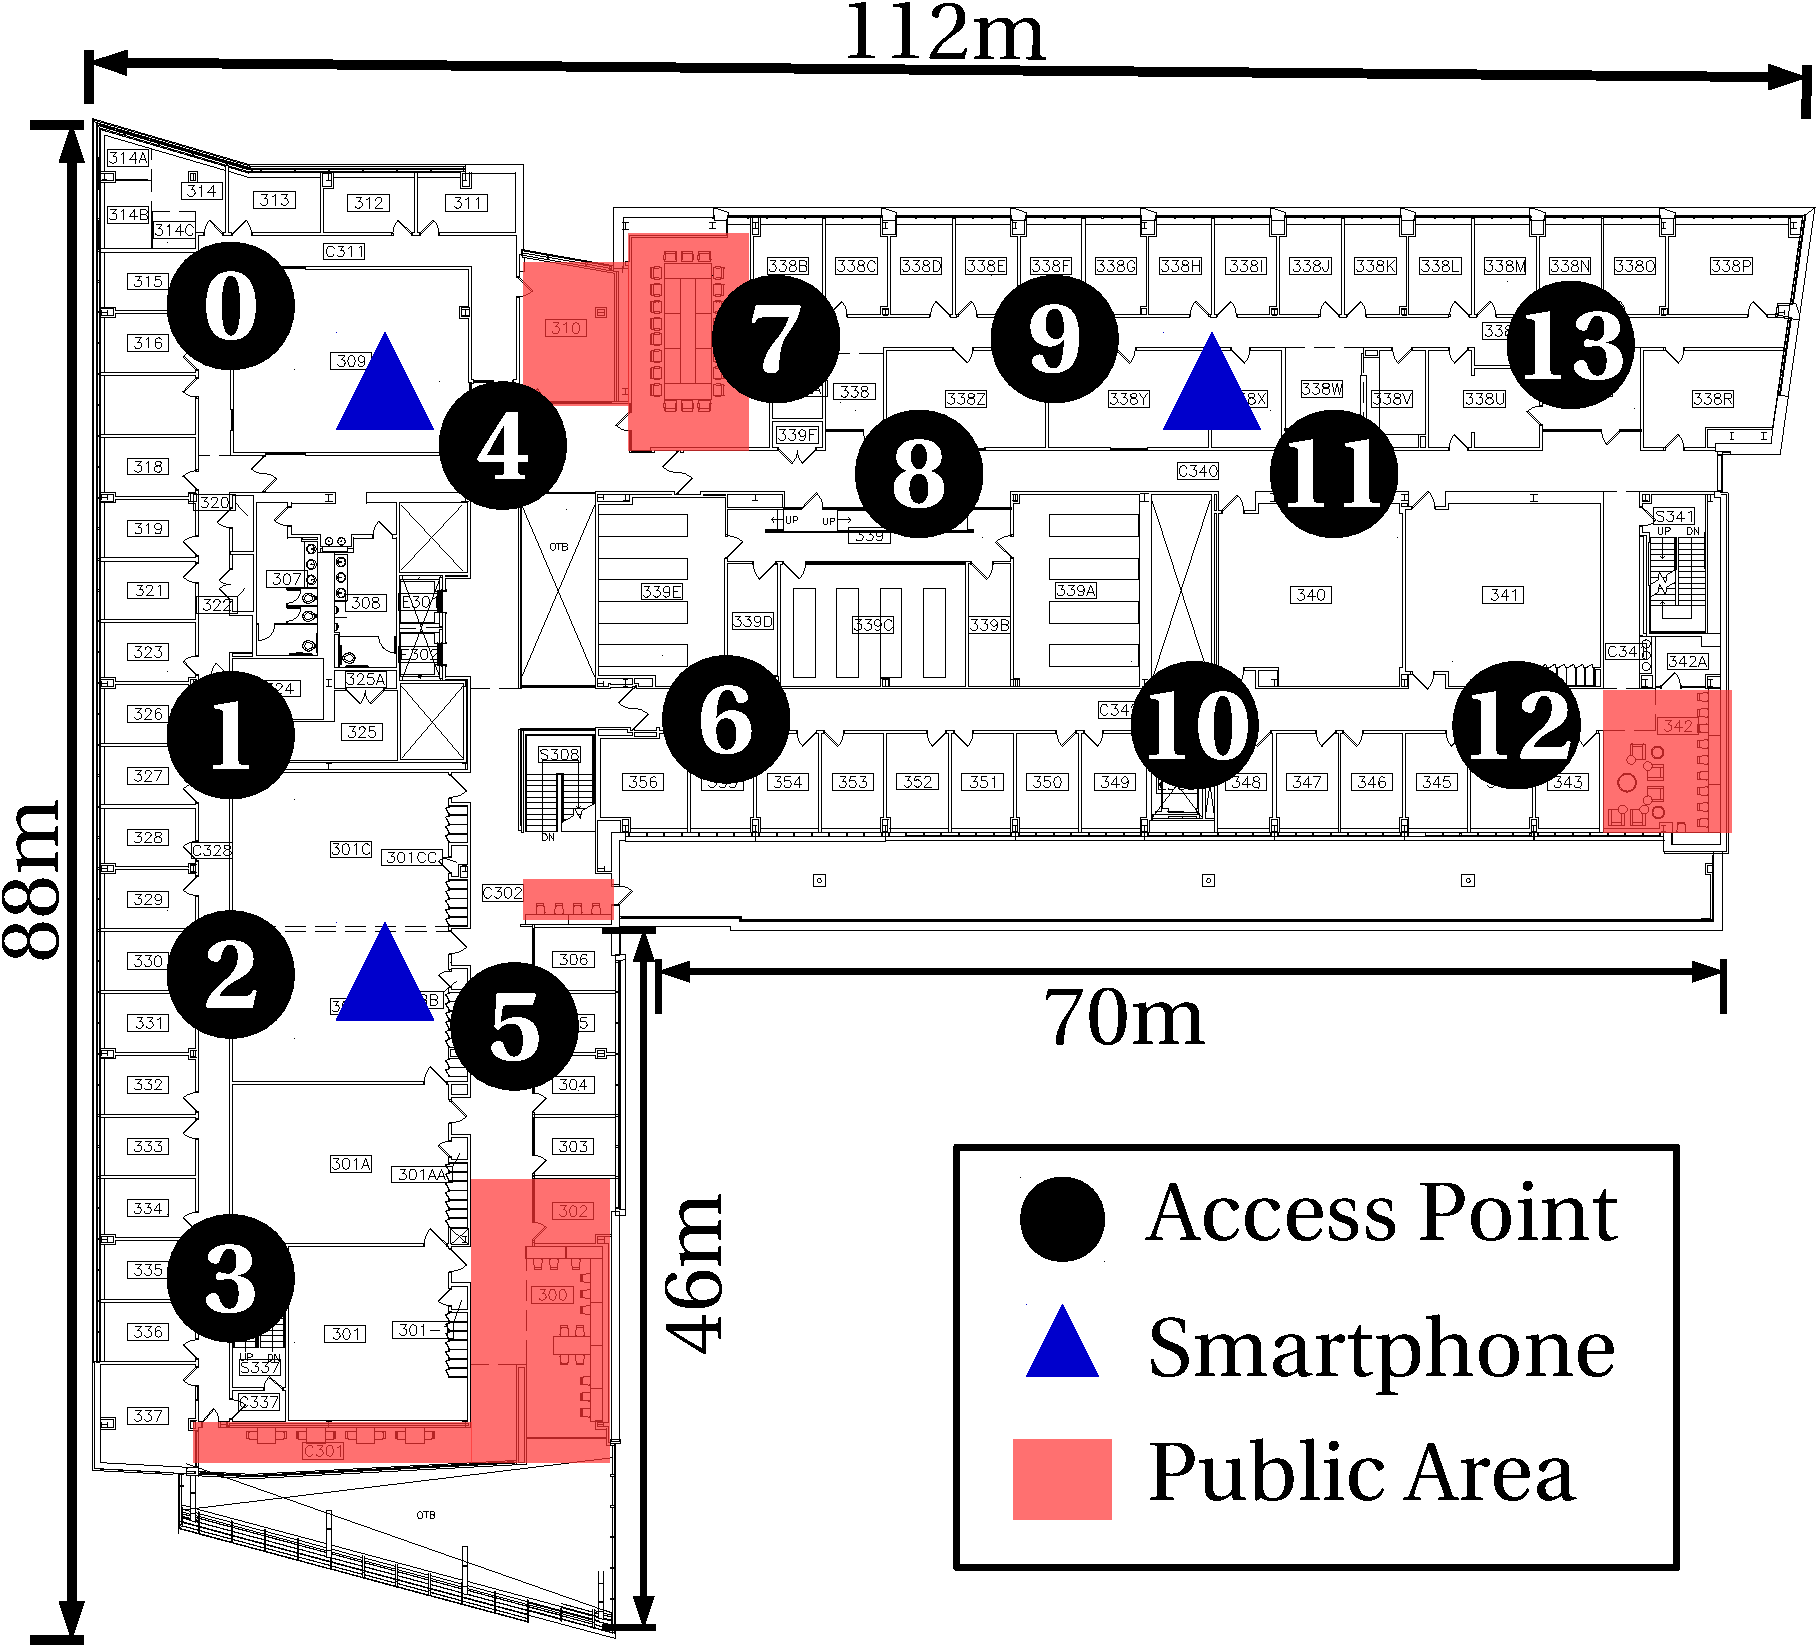
\includegraphics[width=\columnwidth]{./figures/davis_floor_plan.pdf}
    \caption{\textbf{Floor Plan and AP position.}}
    \label{fig:floor}
  \end{minipage}\hspace{0.01\textwidth}%
  \begin{minipage}[t]{0.33\textwidth}
    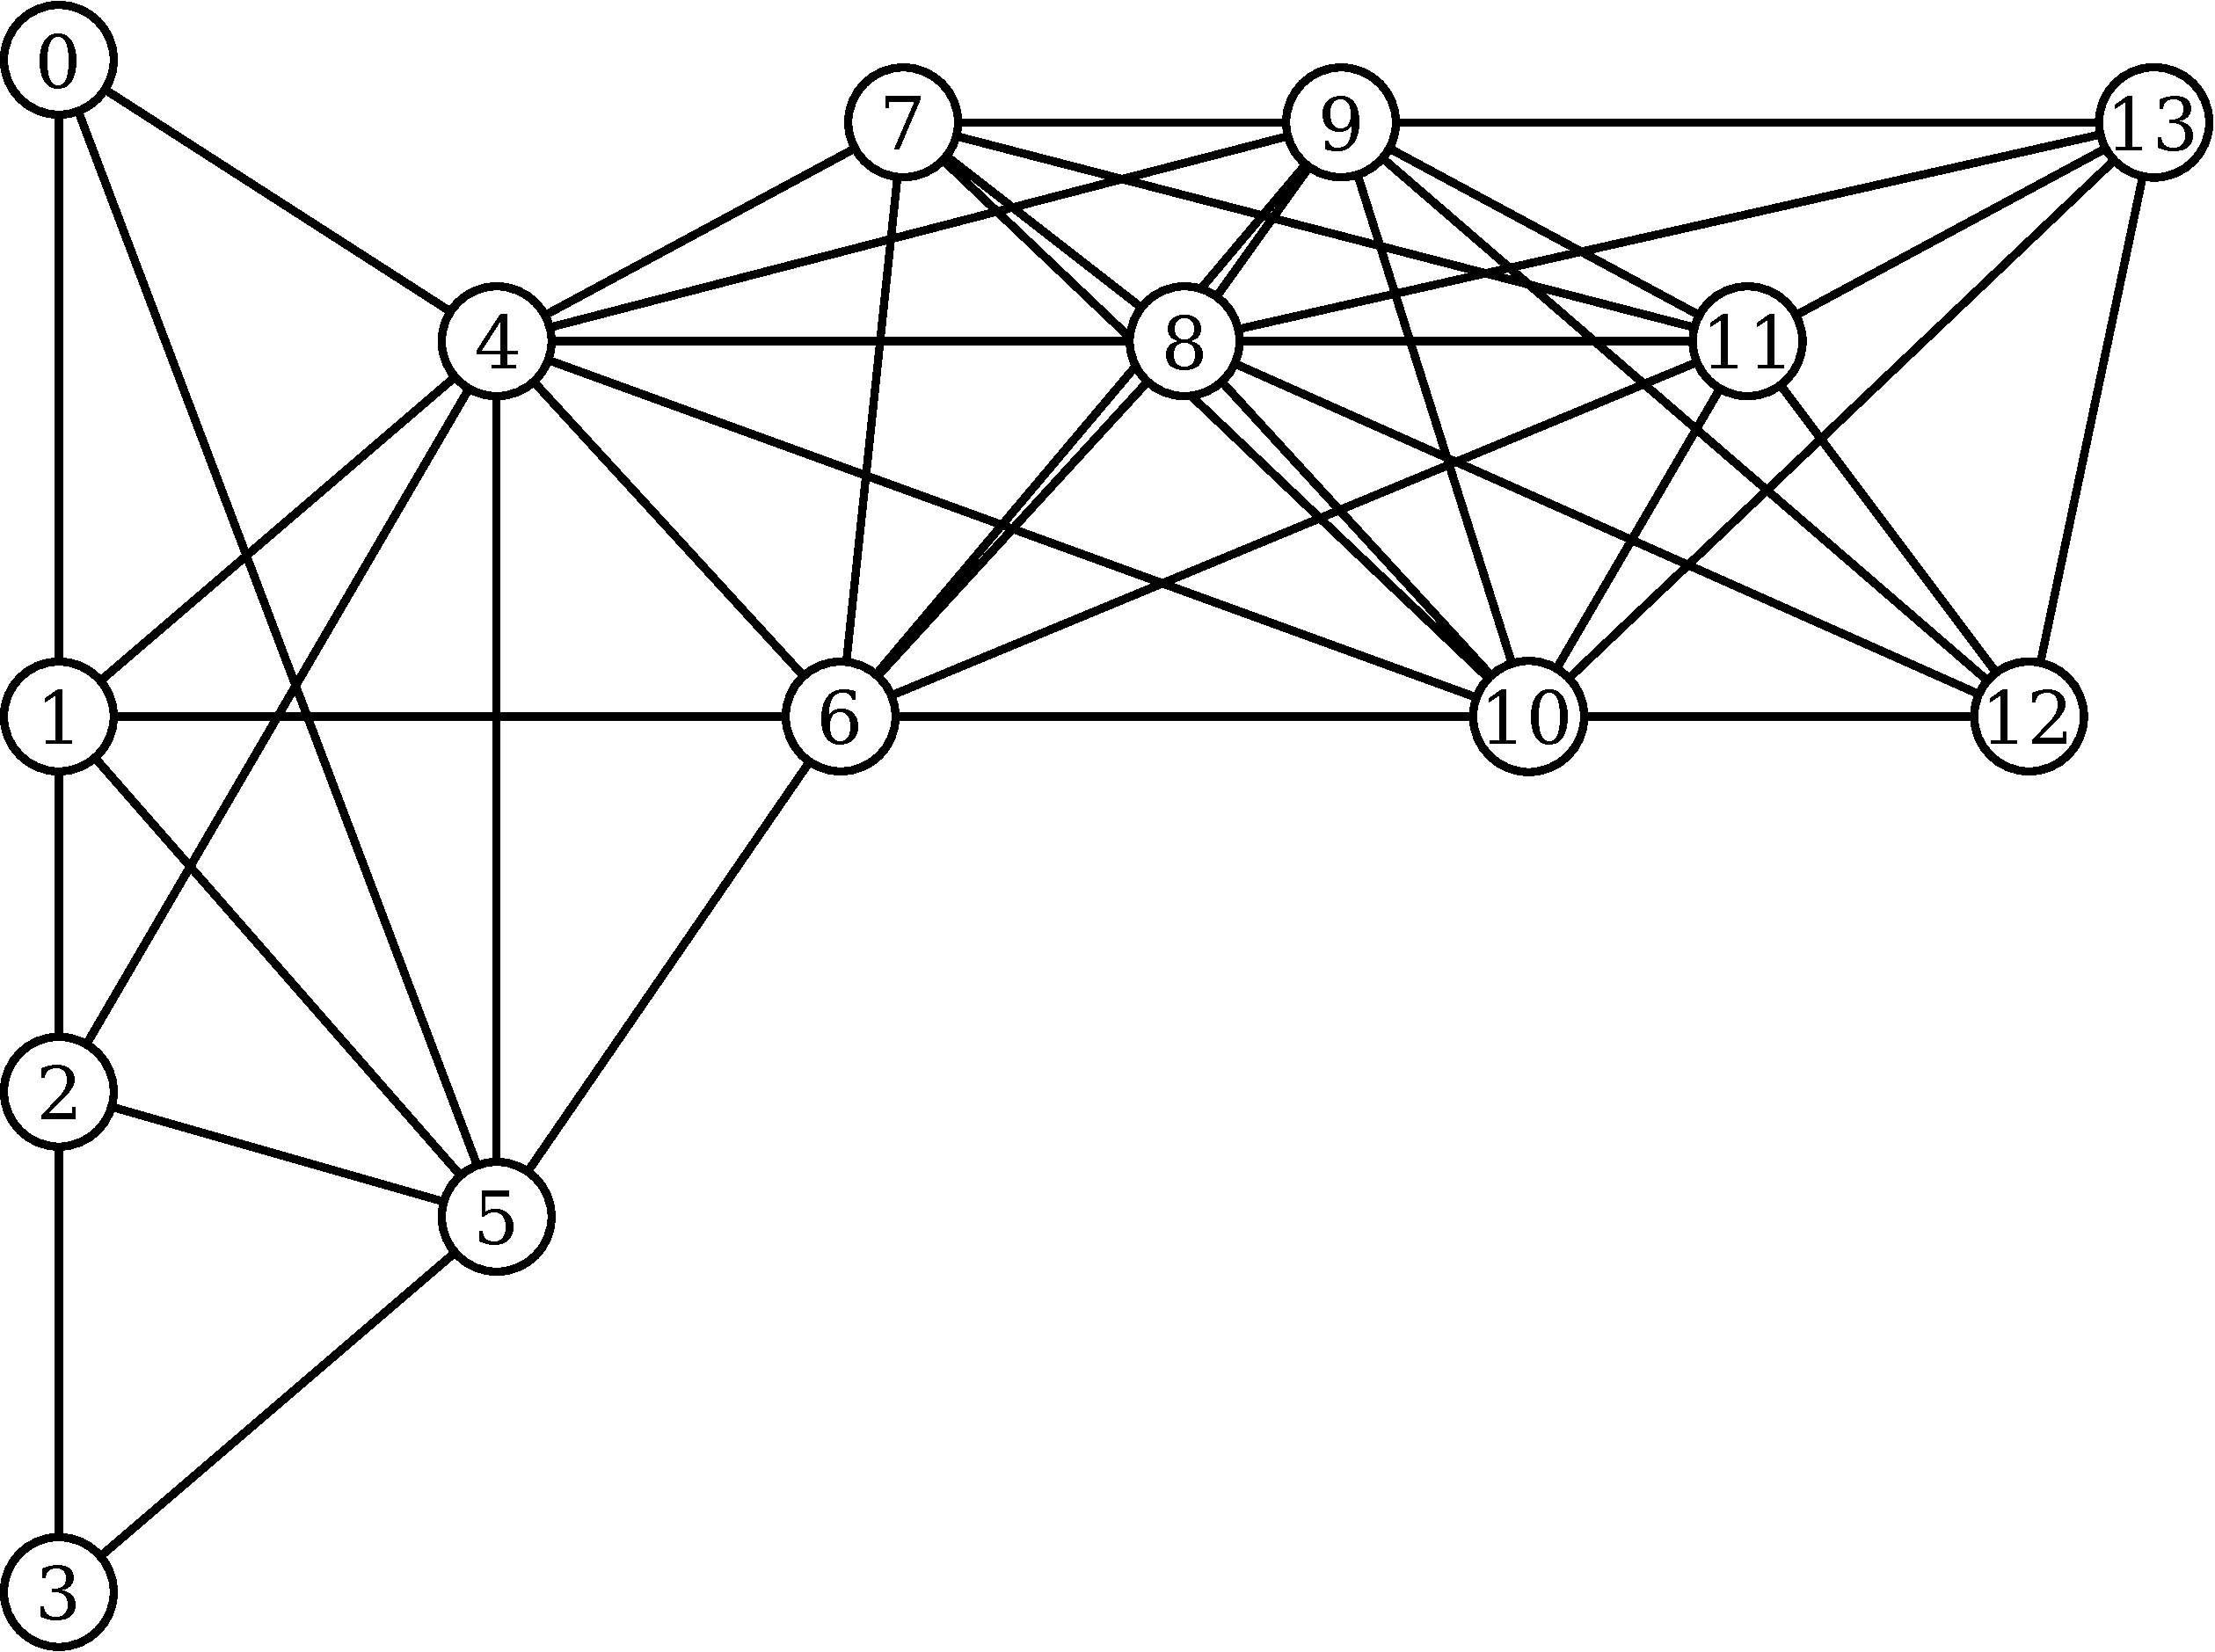
\includegraphics[width=\textwidth]{./figures/DavisConflictGraphSeparate-AP.pdf}
    \caption{\textbf{Infrastructure-perceived Conflict Graph.}}
    \label{fig:ap_conflict}
  \end{minipage}\hspace{0.01\textwidth}%
  \begin{minipage}[t]{0.33\textwidth}
    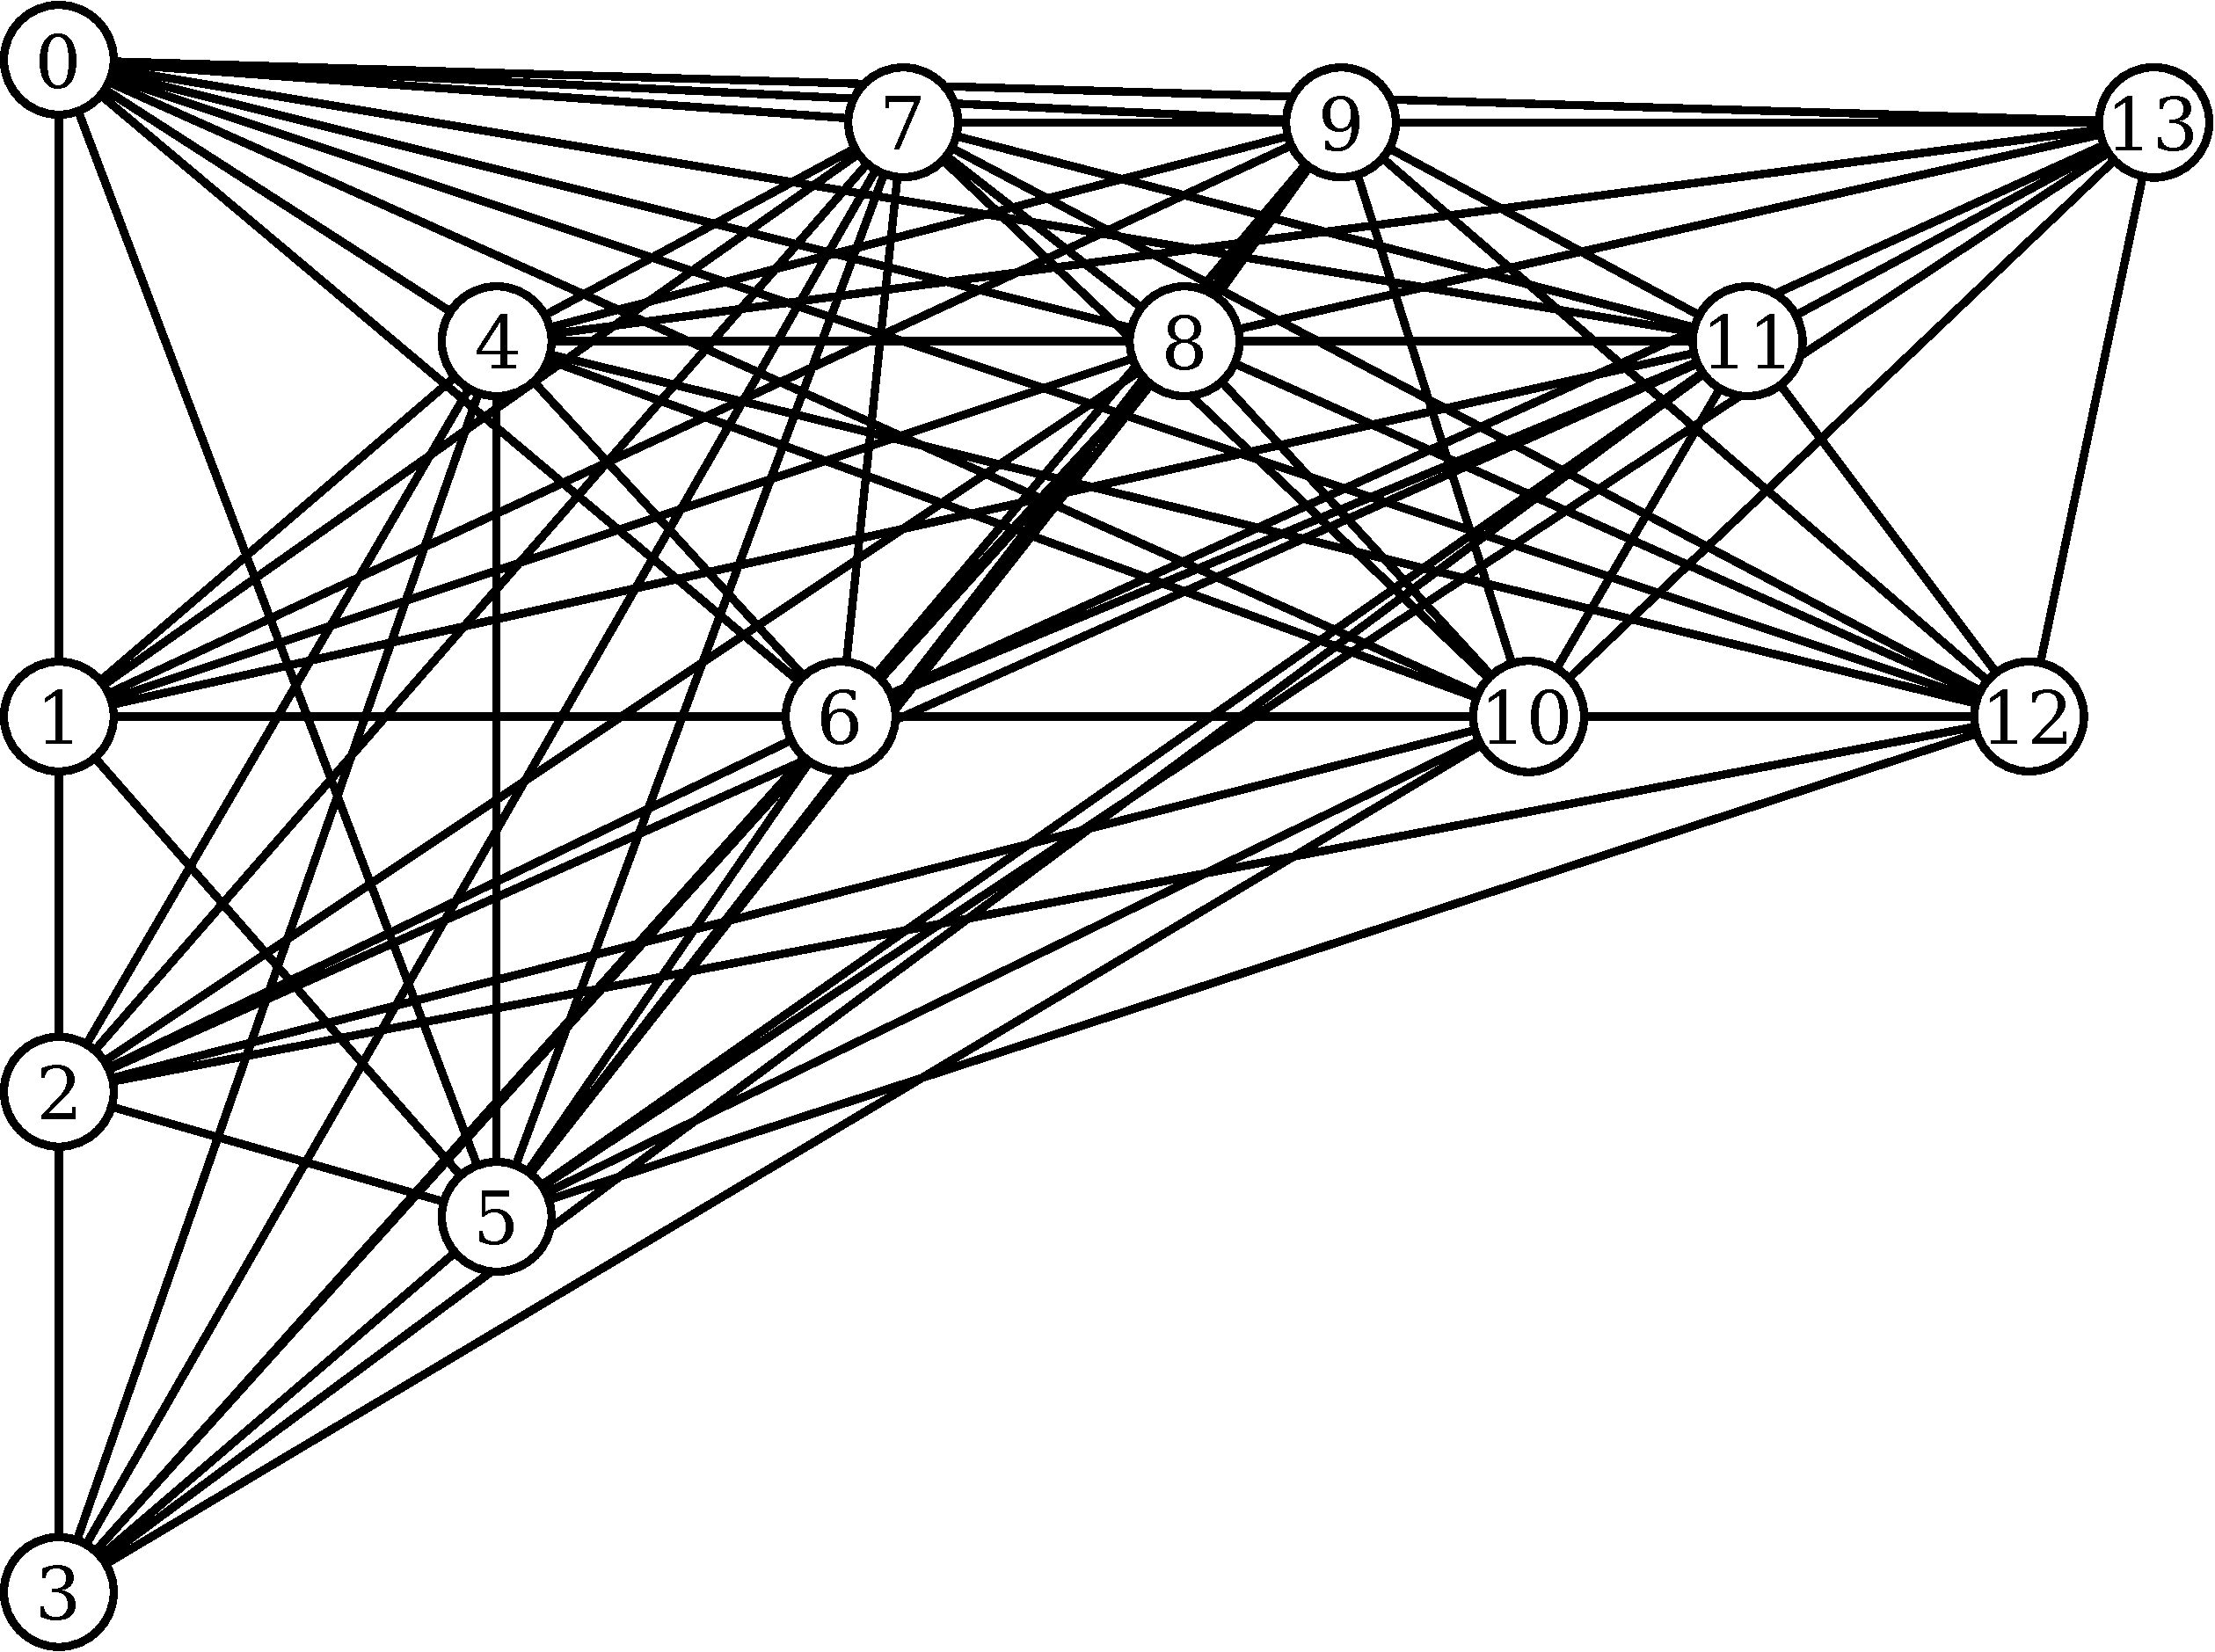
\includegraphics[width=\textwidth]{./figures/DavisConflictGraphSeparate-Client.pdf}
    \caption{\textbf{Client-perceived Conflict Graph.}}
    \label{fig:client_conflict}
  \end{minipage}
  \vspace*{\aftercaptiongap}
\end{figure*}


Channel assignment plays an important role in wireless network performance, and
is typically modeled as a graph coloring problem on conflict graph $G=(V, E)$,
where $V$ is the set of APs, and $\langle AP_i, AP_j \rangle \in E$ if $AP_i$
and $AP_j$ interfere with each other when they are in the same channel. Previous
works~\cite{mishra2005weighted,mishra2006client} have shown that conflict graph
constructed with only AP side measurement fails to capture all types of interference
due to the hidden terminal problems. For instance, suppose
$AP_i$ and $AP_j$ are beyond each other's communication range, with only AP's
measurements, $\langle AP_i, AP_j \rangle \notin E$. However, a client that is
associated with $AP_i$ may still experience interference from $AP_j$.

In this section, we first show how the smartphone measurements can help build a
more representative conflict graph that captures the interference experienced by
clients. Then we demonstrate how to use this conflict graph to reduce
client-perceived conflicts.

\subsubsection{Client-Assisted Conflict Graph Construction}
\label{subsec:client_conflict}

The conflict graph can be constructed with only infrastructure side measurements:
each AP performs a \wifi{} scan and inserts an edge between itself and
each of its neighbors. We refer to a graph constructed in this manner as the
\textit{Infrastructure-perceived} conflict graph, or $G_I=(V, E_I)$, where $V$
is the set of APs, and $\langle AP_i, AP_j \rangle \in E_I$ if $AP_i$ can
overhear $AP_j$'s beacon frame, or vice versa. 

To construct $G_I$, we need the AP-side scan results. Due to the limitation
aforementioned in Section~\ref{subsec:cit}, we are only able to construct $G_I$
for the 14 APs in our department building, as shown in Figure~\ref{fig:floor}.
With the \ubapdetail{} dataset, for each $AP_i$, we add $\langle AP_j, AP_i \rangle$
to $E_I$ if $AP_j$ shows up in $AP_i$'s scan results. Note that in \ubapdetail{}
dataset, we did not find any asymmetric AP pairs, effectively making $G_I$ undirected.

However, from the \wifi{} client's perspective, any AP (other than its currently
associated AP) within its carrier sensing range has potential conflict with
itself, causing either extra backoff delay for uplink packets, or collisions for
downlink packets. Therefore, a more representative conflict graph should also
include edges between the client's associated AP and all other APs that appear
in the client's scan results during the \wifi{} session. We refer to such graph as
\textit{client-perceived} conflict graph, or $G_C=(V, E_C)$, where $V$ is the
set of APs, and $\langle AP_i, AP_j \rangle \in E_C$ if any of $AP_i$'s clients
can overhear beacon frames from $AP_j$, or vice versa.

We use the \ubscan{} dataset to construct $G_C$ as follows. Given a scan
result from a smartphone that was associated with $AP_i$, we add $\langle AP_j,
AP_i \rangle$ to $E_C$ if $AP_j$ appears in the result. We also count the number
of unique $\langle device, timestamp \rangle$%
\footnote{Timestamps are binned by hour---multiple scan results within an hour
from the same device are only counted once towards the edge weight---so the
weight is not  biased by certain busy devices.} %
tuples for each conflict edge as its weight, to quantify the impact of
the conflict: a large weight means the conflict is experienced by many
devices and/or for a long period of time.


Figure~\ref{fig:ap_conflict} and Figure~\ref{fig:client_conflict} show the
constructed infrastructure-perceived and client-perceived conflict graphs
respectively, where APs are positioned by their physical coordinates in
Figure~\ref{fig:floor}. First, we observe that $G_C$ contains many edges that do
not exist in $G_I$, which implies that clients experience more conflicts than
the infrastructure can identify. Second, in this particular AP placement, we
notice that $E_I$ is a \textit{proper subset} of $E_C$, which means our dataset
not only reveals hidden conflicts, but also detects all conflicts that the APs
already see.

We then take a closer look at each node's degree in both conflict graphs.  The
median node degree in $G_I$ is 7, which is not surprising given the dense AP
deployment in this floor.  In $G_C$, the min degree is 10 and the median degree
is 13. In reality, however, not all the conflict edges exist all the time: while
$G_I$ is stable, $G_C$ may vary over time due to client mobility or association
behavior. Therefore, such temporal fluctuations of $G_C$ must be captured to
effectively assign channels without wasting temporal channel reuse
opportunities.

We seek ways to learn such temporal fluctuation patterns using our dataset.
Specifically, we investigate \textit{hourly} patterns. For each edge in
$G_C$, we first obtain the set of unique $\langle device, timestamp \rangle$
tuples that we used to calculate edge weight, then we bin the tuples by the
timestamp's $hour$ field, and thus get the number of tuples in each hour of
day.

\begin{figure*}[t]
  \centering
  \begin{minipage}[b]{0.33\textwidth}
    \vspace*{-1.3cm}
    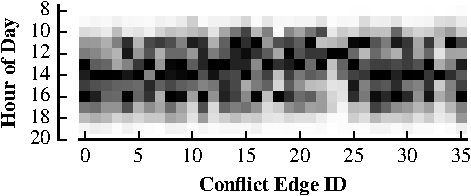
\includegraphics[width=\columnwidth]{./figures/DavisConflictHour.pdf}
    \caption{\textbf{$\langle Device, timestamp \rangle$ Count Distribution for
      Client-Only Conflict Edges.} Hours before 8~AM and after 8~PM are omitted since their counts
      are all near 0. Edges are sorted by their node pair. Each tile are shaded to
      reflect the number of tuples in the hour---darker tile represents more
    conflicts.}
    \label{fig:conflict_hour}
  \end{minipage}\hspace{0.02\textwidth}%
  \begin{minipage}[b]{0.65\textwidth}
    \begin{subfigure}[t]{0.49\textwidth}
      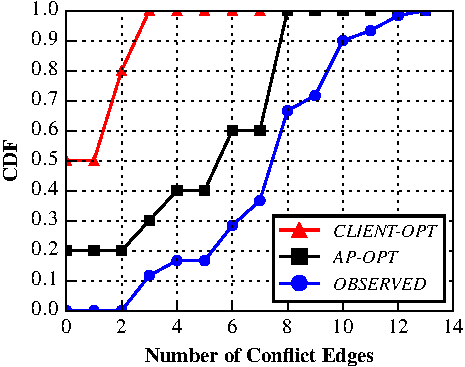
\includegraphics[width=\textwidth]{./figures/DavisConflictEdge.pdf}
      \caption{\textbf{CDF of Conflict Edge Number of Different Channel Assignment.}}
      \label{fig:channel}
    \end{subfigure}\hspace*{0.02\textwidth}%
    \begin{subfigure}[t]{0.49\textwidth}
      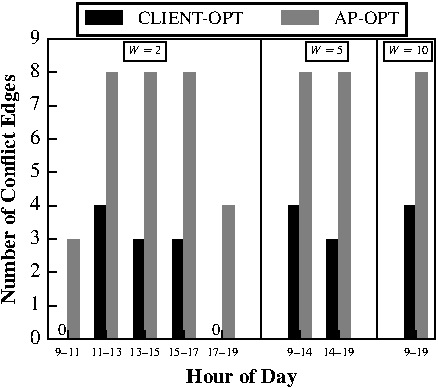
\includegraphics[width=\textwidth]{./figures/DavisConflictEdgeMultiHour.pdf}
      \caption{\textbf{Number of Conflict Edges Over Different Window Size.}}
      \label{fig:window}
    \end{subfigure}
    \caption{\textbf{Channel Assignment on Client- and Infrastructure-Perceived
    Conflict Graph.}}
  \end{minipage}
  \vspace*{\aftercaptiongap}
\end{figure*}



Figure~\ref{fig:conflict_hour} shows the hourly tuple count distribution for
all client-only conflict edges ($E_C-E_I$). As expected, all conflict edges
are mostly seen during school hours (10~AM to 6~PM). Furthermore, different
edges are mostly seen at various hours indicated by the darkest tile of each
conflict edge. With such temporal fluctuation information, we can now
construct the time-variant $G_C(h)=(V, E_C(h))$, where $h$ is a given hour of
day, and $E(h)$ contains all the stable edges plus the edges that are
reported at time $h$.


\subsubsection{Channel Assignment}

We then look at the effects of hidden conflict edges to the channel assignment
of campus APs. According to \ub{} IT staff, all campus APs are connected to
central controllers, which collect the interference information from the APs and
adjust each APs' channel to reduce conflicts. However, the measurement process
and the channel assignment algorithm are all handled behind the scene, and
little details were revealed or documented. Therefore, we again focus on
the campus APs in our department building.

To monitor the APs' operating channels, we placed three smartphones in locations
marked as triangles in Figure~\ref{fig:floor}, and verified that the smartphones
together can see all 14 APs in this floor. We configure the smartphones to
perform a \wifi{} scan periodically. The experiment lasted for 6 days from Apr
23 to Apr 28, 2015. We fused the data from all devices and obtain each AP's
channel history during the experiment period. In total, we detected no channel
switch events in the 2.4~GHz band and 157 switch events in the 5~GHz band, which
suggests the campus controllers only try to adapt channels in the 5~GHz band.
Therefore, we hereby focus on the 5~GHz band only.

There are 9 orthogonal channels available in the 5~GHz band in United States. We
verified that the conflict graph $G_I$ for the 14 APs is at least 7 colorable
using the \textit{largest first} strategy described
in~\cite{kosowski2004classical}.  However, we still observed channel conflicts
among the 14 APs during the experiment period. This is probably because those APs
also have conflicts with campus APs in other floors, thus the actual conflict
graph is larger than $G_I$ we constructed.

We compare three channel assignment schemes: the observed channel assignment by
campus AP controllers (\textit{OBSERVED}), optimal channel assignment on $G_I$
(\textit{AP-OPT}) alone, and optimal channel assignment on $G_C(h)$
(\textit{CLIENT-OPT}). For each scheme, we calculate the number of conflicts on
$G_C(h)$ for each school hour (8~AM--6~PM) during our experiment period. This
metric captures the actual number of conflicts experienced by the clients.

Figure~\ref{fig:channel} shows the CDF of number of conflicts of all 60 school-hours
(10 hours/day$\times$6 days). We can see that when considering only $G_I$, both the
controller (\textit{OBSERVED}) and even the optimal channel assignment
(\textit{AP-OPT}) cause many conflicts from client's perspective. With client's
feedback, however, an optimal channel assignment on $G_C$ (\textit{CLIENT-OPT})
can be conflict free 50\% of the time, and no more than 3 conflict edges
at any time.


In practice, controllers may not be able to reassign channels as frequently as
once
per hour. Therefore, we extend the analysis to longer intervals. For a time
window of $W (W>1)$ hours, we obtain the conflict graph by combining the
conflict edges from each hour in the time window. We then compare the number of
conflicts of \textit{AP-OPT} and \textit{CLIENT-OPT} scheme.
Figure~\ref{fig:window} shows the results for $W=2, 5, \text{ and } 10$
respectively. As expected, both coloring schemes incur more conflicts than
single hour case, since there are more edges in the graph to be colored.
However, \textit{CLIENT-OPT} can achieve significantly fewer conflicts than
\textit{AP-OPT}.

\subsubsection{Campus Network Conflict Graph}

We now examine the entire campus wireless network. The goal is to understand
the complexity of large scale production wireless network deployments. We
first construct campus wide $G_C$ using the method described in
Section~\ref{subsec:client_conflict}. Figure~\ref{fig:campus_edge_weight}
shows the CDF of edge weight for both \ub{} and \nd{}. Most conflict edges are seen
rarely for both campuses, as both testbeds' participants only constitute a
tiny portion of the entire campus population---0.5\% for \nd{}, and 0.6\% for
\ub{}. To obtain more meaningful insights, we hereafter filter out conflict
edges that are seen less than 10 times.

Figure~\ref{fig:campus_node_degree} shows the CDF of node degree after
filtering. The median degrees are 3 for \nd{} and 5 for \ub{}, thus the AP
deployments at most of the campus areas seem not as dense as our department
building, where the median conflict degree is 13. Again, these results may be
biased by our small sample. We expect more conflict edges to be discovered with
increased user coverage.

Even with such small user samples, however, there are certain APs with high
conflict degrees in both campuses. For instance, at \ub{}, 5\% of APs ($\sim$90)
have degrees larger than 20, posing challenges to spectrum management in such
dense environments. Temporal patterns can be learned for such APs to discover
channel reuse opportunities.


\subsubsection{Discussion}

Using the datasets, we demonstrate that the measurements from smartphones can
help build a more representative conflict graph and do better channel
assignment. Furthermore, patterns can be learned from longitudinal
measurements to adapt for temporal fluctuations in order to discover channel
reuse opportunities.

Note that it is also possible to collect client slide conflict information in
real time. For instance, 802.11k Radio Resource Measurement (RRM)
amendment~\cite{80211k} defines a measurement type called \textit{Frame
Report}, in which the AP asks the client to report the number of packets the
client receives from each unique transmitter on all channels. The AP can then
use this information to infer other APs within the client's vicinity.
However, such active measurements are disruptive since they require the
client to switch channels.

\begin{figure*}[t]
  \centering
  \begin{minipage}[b]{0.65\textwidth}
    \begin{subfigure}[t]{0.48\textwidth}
      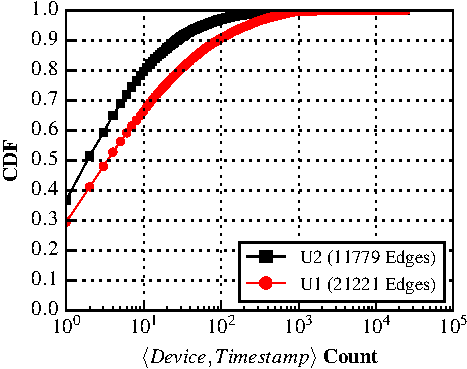
\includegraphics[width=\columnwidth]{./figures/CampusConflictWeight.pdf}
      \caption{\textbf{CDF of Edge Seen Count.} Timestamps are binned by hour. 50\%
      of edges are seen less than 2 (\nd{}) or 3 (\ub{}) times.}
      \label{fig:campus_edge_weight}
    \end{subfigure}\hspace{0.02\textwidth}%
    \begin{subfigure}[t]{0.48\textwidth}
      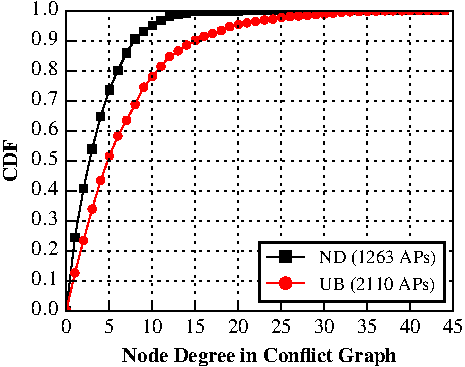
\includegraphics[width=\columnwidth]{./figures/CampusConflictDegree.pdf}
      \caption{\textbf{CDF of Node Degree.} Edges seen less than 10 times are
      ignored.}
      \label{fig:campus_node_degree}
    \end{subfigure}%
    \caption{\textbf{Characteristics of Campus-Wide Conflict Graph.}}
  \end{minipage}\hspace{0.01\textwidth}
  \begin{minipage}[b]{0.33\textwidth}
    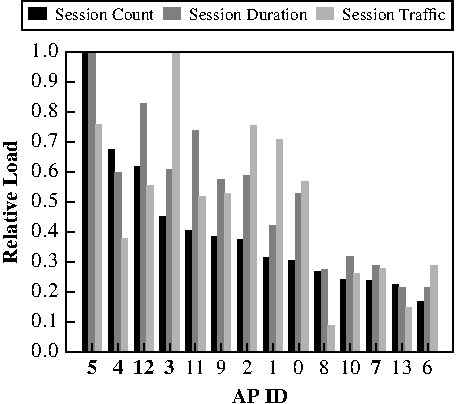
\includegraphics[width=\textwidth]{./figures/DavisAPLoad.pdf}
    \caption{\textbf{Relative AP Load in Department Building.} Each load metric
      is normalized by the maximum value in that category.}
    \label{fig:load}
  \end{minipage}
  \vspace*{\aftercaptiongap}
\end{figure*}

